\documentclass[a4paper,11pt]{article}
\usepackage[T1]{fontenc}
\usepackage[utf8]{inputenc}
\usepackage{lmodern}
\usepackage[british]{babel}
\usepackage{graphicx}

\usepackage{csquotes}
\usepackage{subcaption}
\usepackage[section]{placeins}
\title{}
\author{}

\begin{document}

%\maketitle
%\tableofcontents
\section*{{\LARGE FCA Tool}}
\section{Purpose}
The FCA Tools is a web-based application implemented as an elgg plug-in that allows the creation of knowledge domains consisting of concepts based on attributes mapped to objects. The underlying principle is based on Formal Concept Analysis (FCA). The FCA Tool consists of two parts. An \emph{editor view} presenting a matrix that allows the creation of knowledge domains by associating attributes to objects and a \emph{lattice view} containing a graph representation of a domain consisting of interconnected concepts. The computation of the graph as well as persistent storage, is handled by a back-end service. Therefore a persistent internet connection is required since the user facing part cannot function on its own.
\section{User Interface}
When launching the FCA Tool the initial screen as depicted in Figure \ref{fig:fca-init} is presented consisting of two main parts: the menu bar \textbf{[F01]} and the workspace \textbf{[F02]}.\\
\begin{figure}[h]
\begin{center}
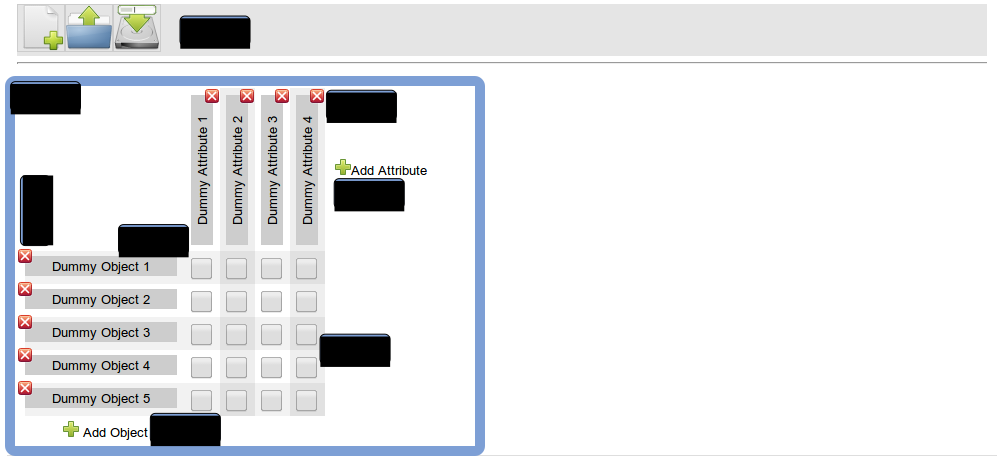
\includegraphics[width=0.8\textwidth]{figures/01_main}  
\end{center}
\caption{Initial view}
\label{fig:fca-init}
\end{figure}

The menu bar buttons allow for creating a new domain (discarding all unsaved changes), opening existing domains (also discarding all changes) and saving the current state as a new domain.
The concept of editing an existing domain is implemented as simply saving the current state as a new domain leaving already existing domains unchanged.

The purpose of the workspace is to create objects, attributes, learning objects and assemble them to knowledge domains. This interface section consists of the following elements:
Object-- and attribute buttons \textbf{[F02.1]}  represeniting objects and attributes as rows and columns of a matrix. Upon clicking these buttons a dialogue window is presented allowing to choose from existing objects/attributes or create new ones. Using
  buttons to add objects and attributes \textbf{[F02.2]} the overall number of objects/attributes can be increased while
  removal buttons \textbf{[F02.3]} allow for deleting individual objects and attributes.
  Objects are associated to attributes by ticking the corresponding
  checkboxes \textbf{[F02.4]}.
  
\subsection{Selecting Attributes}
(This section also applies to objects.)\\
After clicking an attribute button the dialogue as shown in Figure \ref{fig:fca-attr-set} opens, presenting a combo box \textbf{[F03.1]} allowing to either choose from existing attributes or create a new one. A choice can be acknowledged or cancelled using the control buttons at the bottom of the dialogue window \textbf{[F03.0]}.
%
\begin{figure}[h]
\begin{center}
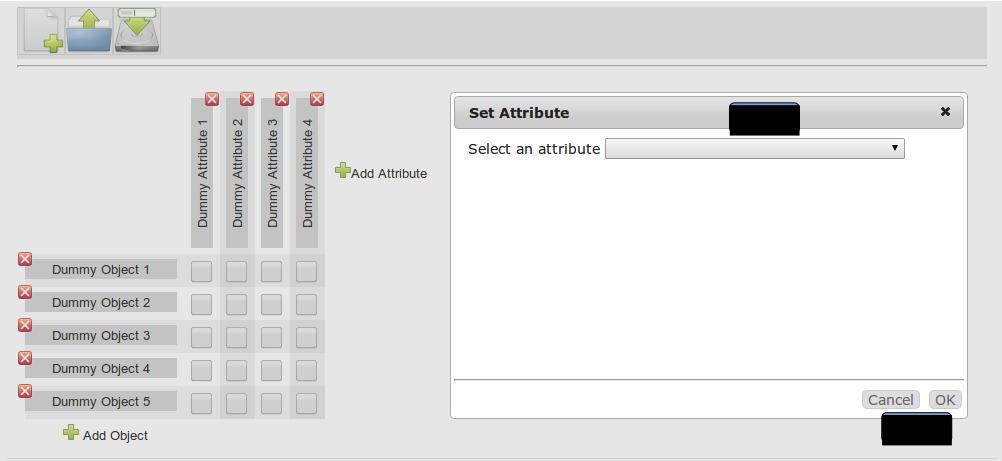
\includegraphics[width=0.8\textwidth]{figures/attr_sel}  
\end{center}
\caption{Set Attribute Dialogue}
\label{fig:fca-attr-set}
\end{figure}
\begin{figure}[h]
\begin{center}
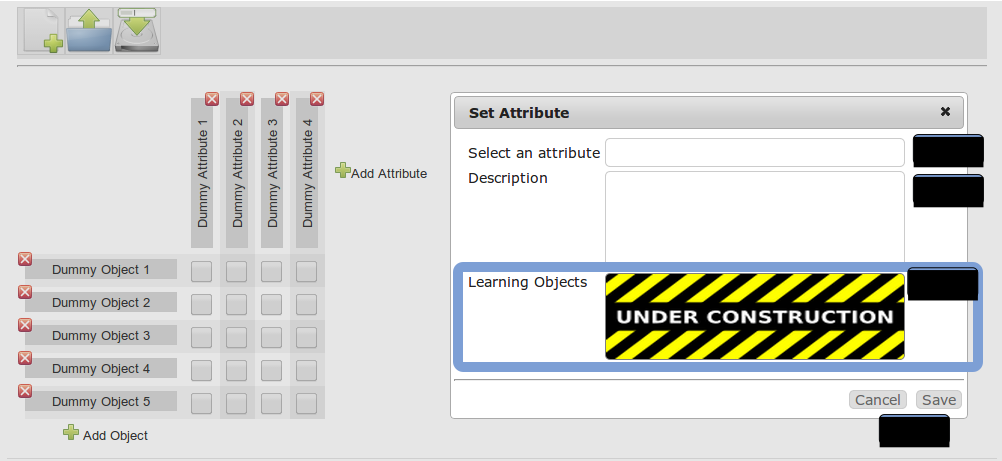
\includegraphics[width=0.8\textwidth]{figures/attr_new}  
\end{center}
\caption{Create Attribute Dialogue}
\label{fig:fca-attr-new}
\end{figure}
%
\paragraph*{Creating New Attributes\\}
When choosing to create a new attribute (by selecting the bottom-most choice available from the combo box) new elements become available (see Figure \ref{fig:fca-attr-new}). Text fields to enter an attribute name \textbf{[F03.2]} and description \textbf{[F03.3]} as well as an area reserved for learning objects \textbf{[F03.4]} that allows for assigning learning objects to this attribute once it is saved. Using the aforementioned control buttons \textbf{[F03.0]} the newly created attribute can either be saved or discarded.
\paragraph*{Choosing Existing Attributes\\}
When selecting an existing attribute through the combo box \textbf{[F03.1]} its description (if any) and learning objects associated to it are displayed (if any) as shown in Figure \ref{fig:fca-attr-show}. Furthermore a button to edit the attribute's name and description \textbf{[F03.5]} is available. Editing is performed using the same controls used to create a new attribute (see Figure \ref{fig:fca-attr-edit}).
Another button to associate learning objects to the current attribute \textbf{[F03.6]} is also present. The control button labelled \emph{OK} at the bottom of the dialogue \textbf{[F03.0]} acknowledges the current choice of attribute.
\begin{figure}[h]
\begin{center}
  \begin{subfigure}{0.8 \textwidth}
    \begin{center}
    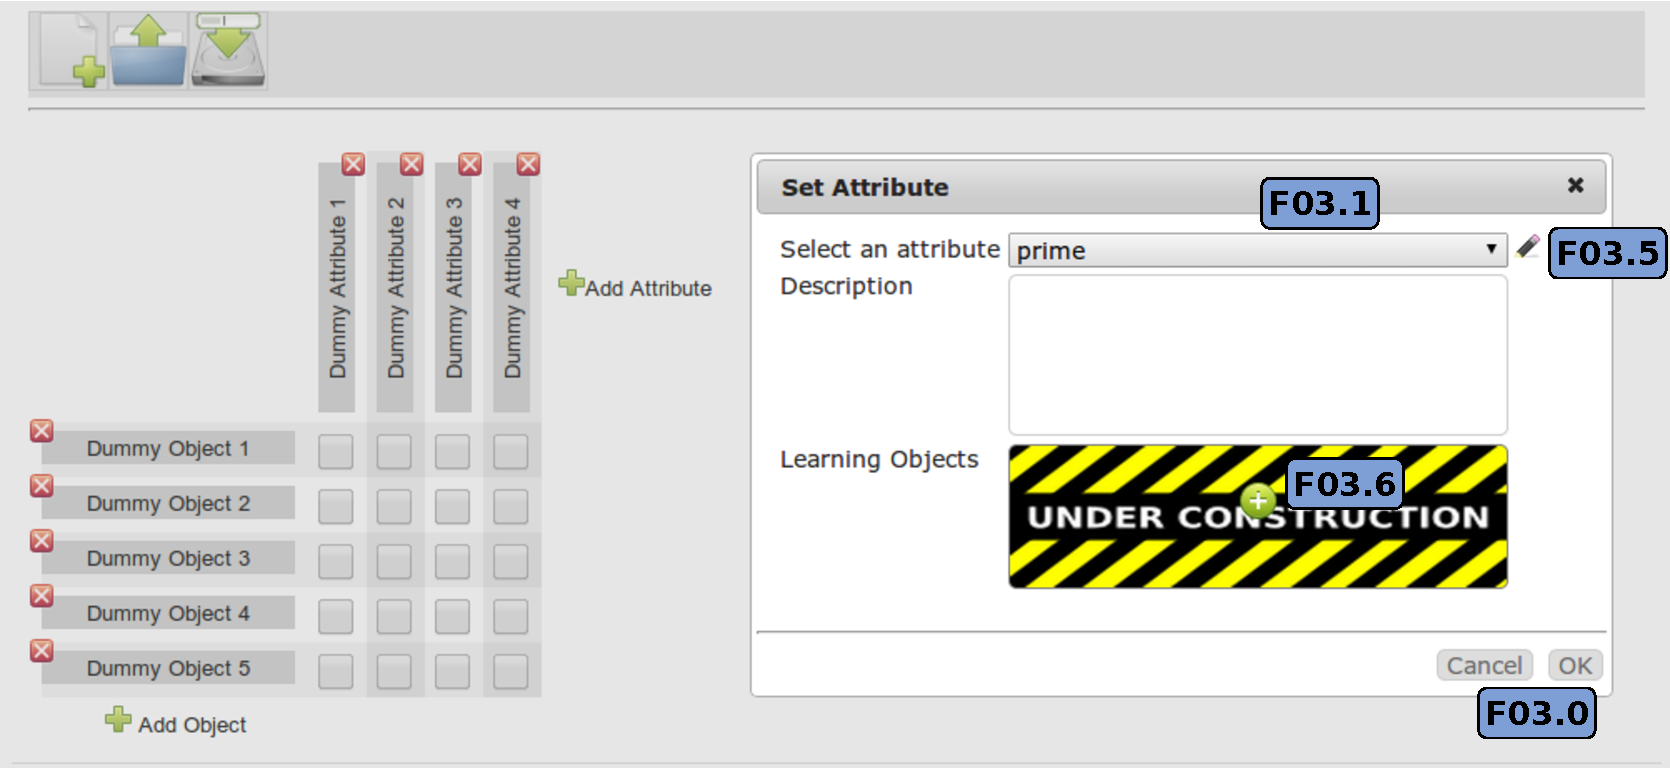
\includegraphics[width=\textwidth]{figures/attr_sow}
    \caption{Attribute Properties}
    \label{fig:fca-attr-show}
    \end{center}
  \end{subfigure}
  \begin{subfigure}{0.8 \textwidth}
    \begin{center}
    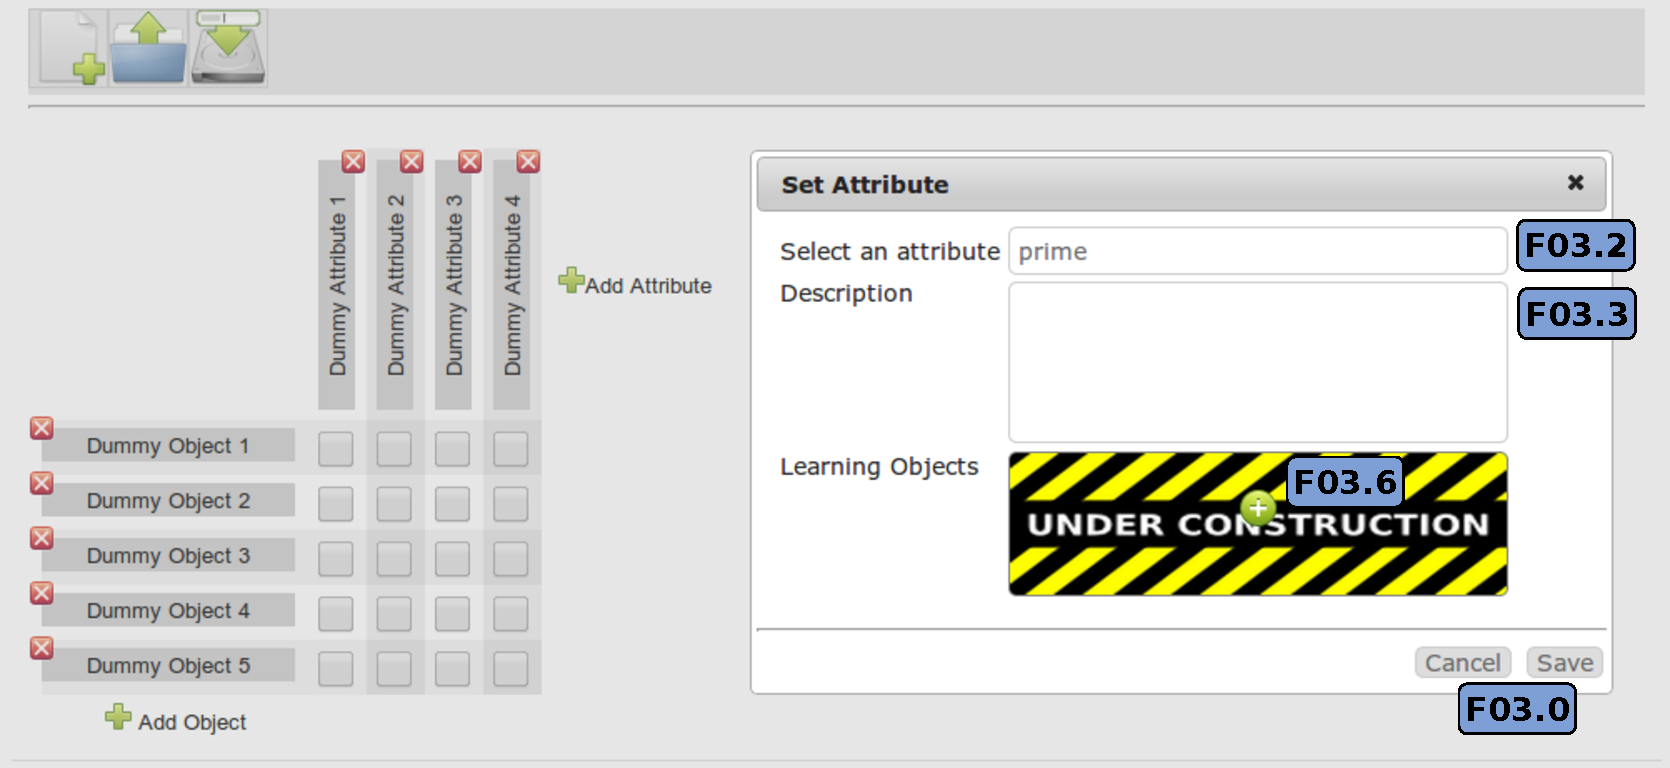
\includegraphics[width=\textwidth]{figures/attr_edit}
    \caption{Attribute Editor}
    \label{fig:fca-attr-edit}
    \end{center}
  \end{subfigure}
\end{center}
\caption{Selecting and Editing an Attribute}
\end{figure}
\subsection{Managing Learning Objects}
(under construction)\\
Associating learning objects to attributes and objects is initiated using button \textbf{[F03.6]} as described previously. This opens another dialogue (see Figure \ref{fig:fca-lo-sel}) similar to the already discussed attribute dialogue shown in Figure \ref{fig:fca-attr-set} that allows for selecting existing learning objects or creating new ones in the same manner by simply choosing an item from the combo box.
\begin{figure}[h]
\begin{center}
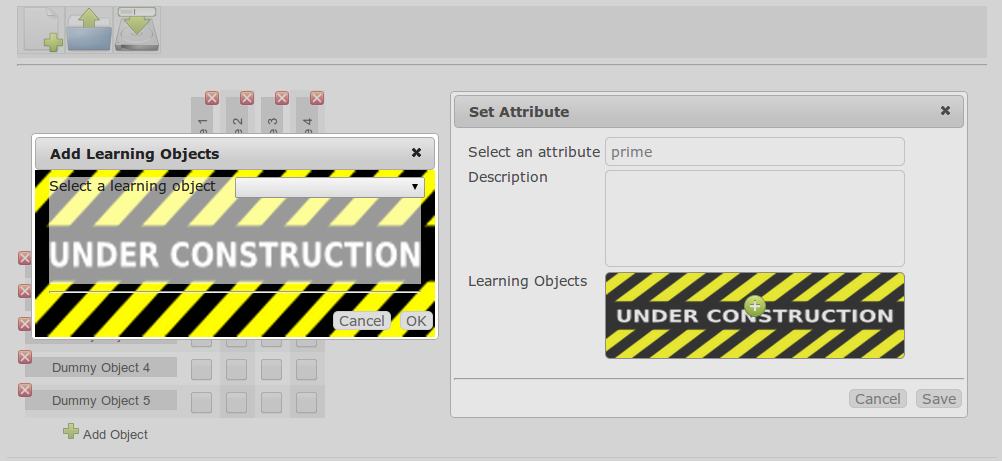
\includegraphics[width=0.8\textwidth]{figures/lo_sel}  
\end{center}
\caption{Select Learning Object Dialogue}
\label{fig:fca-lo-sel}
\end{figure}
\paragraph*{Creating Learning Objects\\}
When creating a learning object a name and a URL to a resource (currently only websites are supported) has to be entered. After this the learning object can be saved and then chosen to be associated to the currently active attribute/object through the combo box of the previously described learning object dialogue. When a choice was made the learning object appears in the list of learning objects of the attribute dialogue as an interactive element \textbf{[F03.7]} (see Figure \ref{fig:fca-attr-lo}). Learning objects can be clicked opening a new browser tab presenting the resource the learning object points to.

When hovering a learning object two new controls appear (see Figure \ref{fig:fca-attr-lo-hover}) allowing to edit (not implemented yet) its properties or removing it from the currently active attribute/object (without deleting it) \textbf{[F03.8]}.
\begin{figure}[h]
\begin{center}
  \begin{subfigure}{0.8 \textwidth}
    \begin{center}
    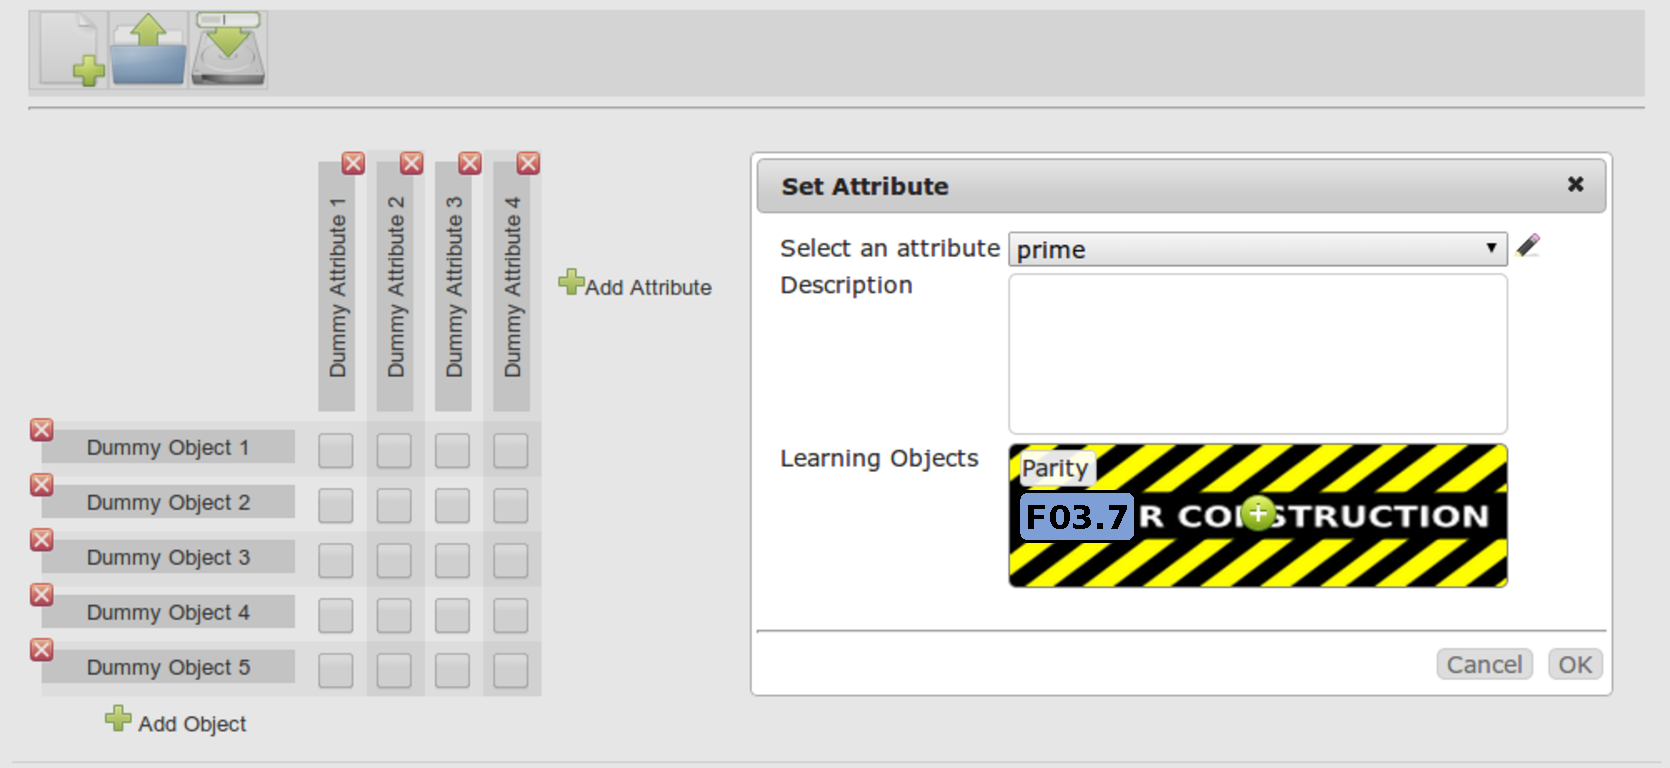
\includegraphics[width=\textwidth]{figures/attr_lo}
    \caption{Learning Object}
    \label{fig:fca-attr-lo}
    \end{center}
  \end{subfigure}
  \begin{subfigure}{0.8 \textwidth}
    \begin{center}
    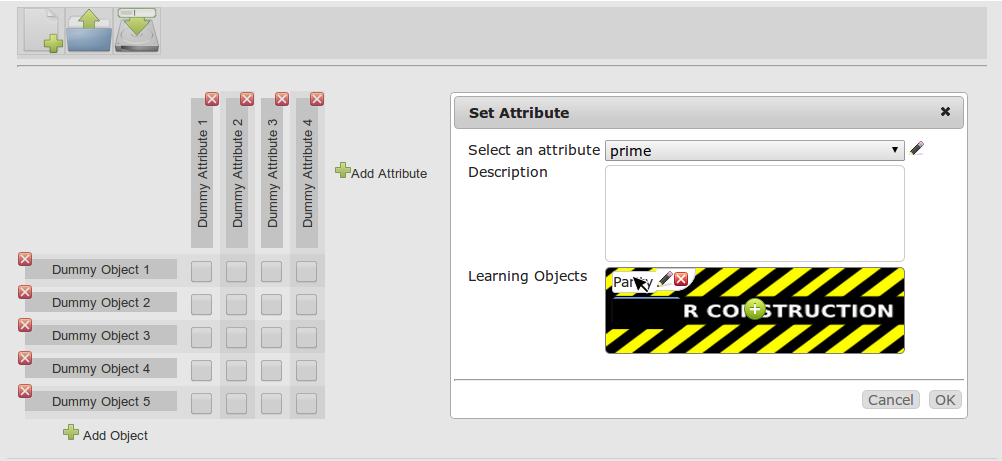
\includegraphics[width=\textwidth]{figures/attr_lo_hov}
    \caption{Learning Object (highlighted)}
    \label{fig:fca-attr-lo-hover}
    \end{center}
  \end{subfigure}
\end{center}
\caption{Interactive Learning Object List}
\end{figure}

\FloatBarrier
\subsection{Lattice View}
After saving or opening a domain a dialogue containing the \emph{lattice view} is presented allowing to interact with a graph representation of the domain (\emph{formal context}) comprised of interconnected formal concepts (see Figure \ref{fig:fca-lattice-view}). The lattice view itself is divided into two parts: A graph section \textbf{[F04]} and a side pane \textbf{[F05]}. Initially a select subset of the formal context -- the taxonomy of the domain -- is presented. The top left check box \textbf{[F04.1]} allows to switch between taxonomy and complete formal context (see Figure \ref{fig:fca-lattice}).
\begin{figure}[h]
\begin{center}
  \begin{subfigure}{0.8 \textwidth}
    \begin{center}
    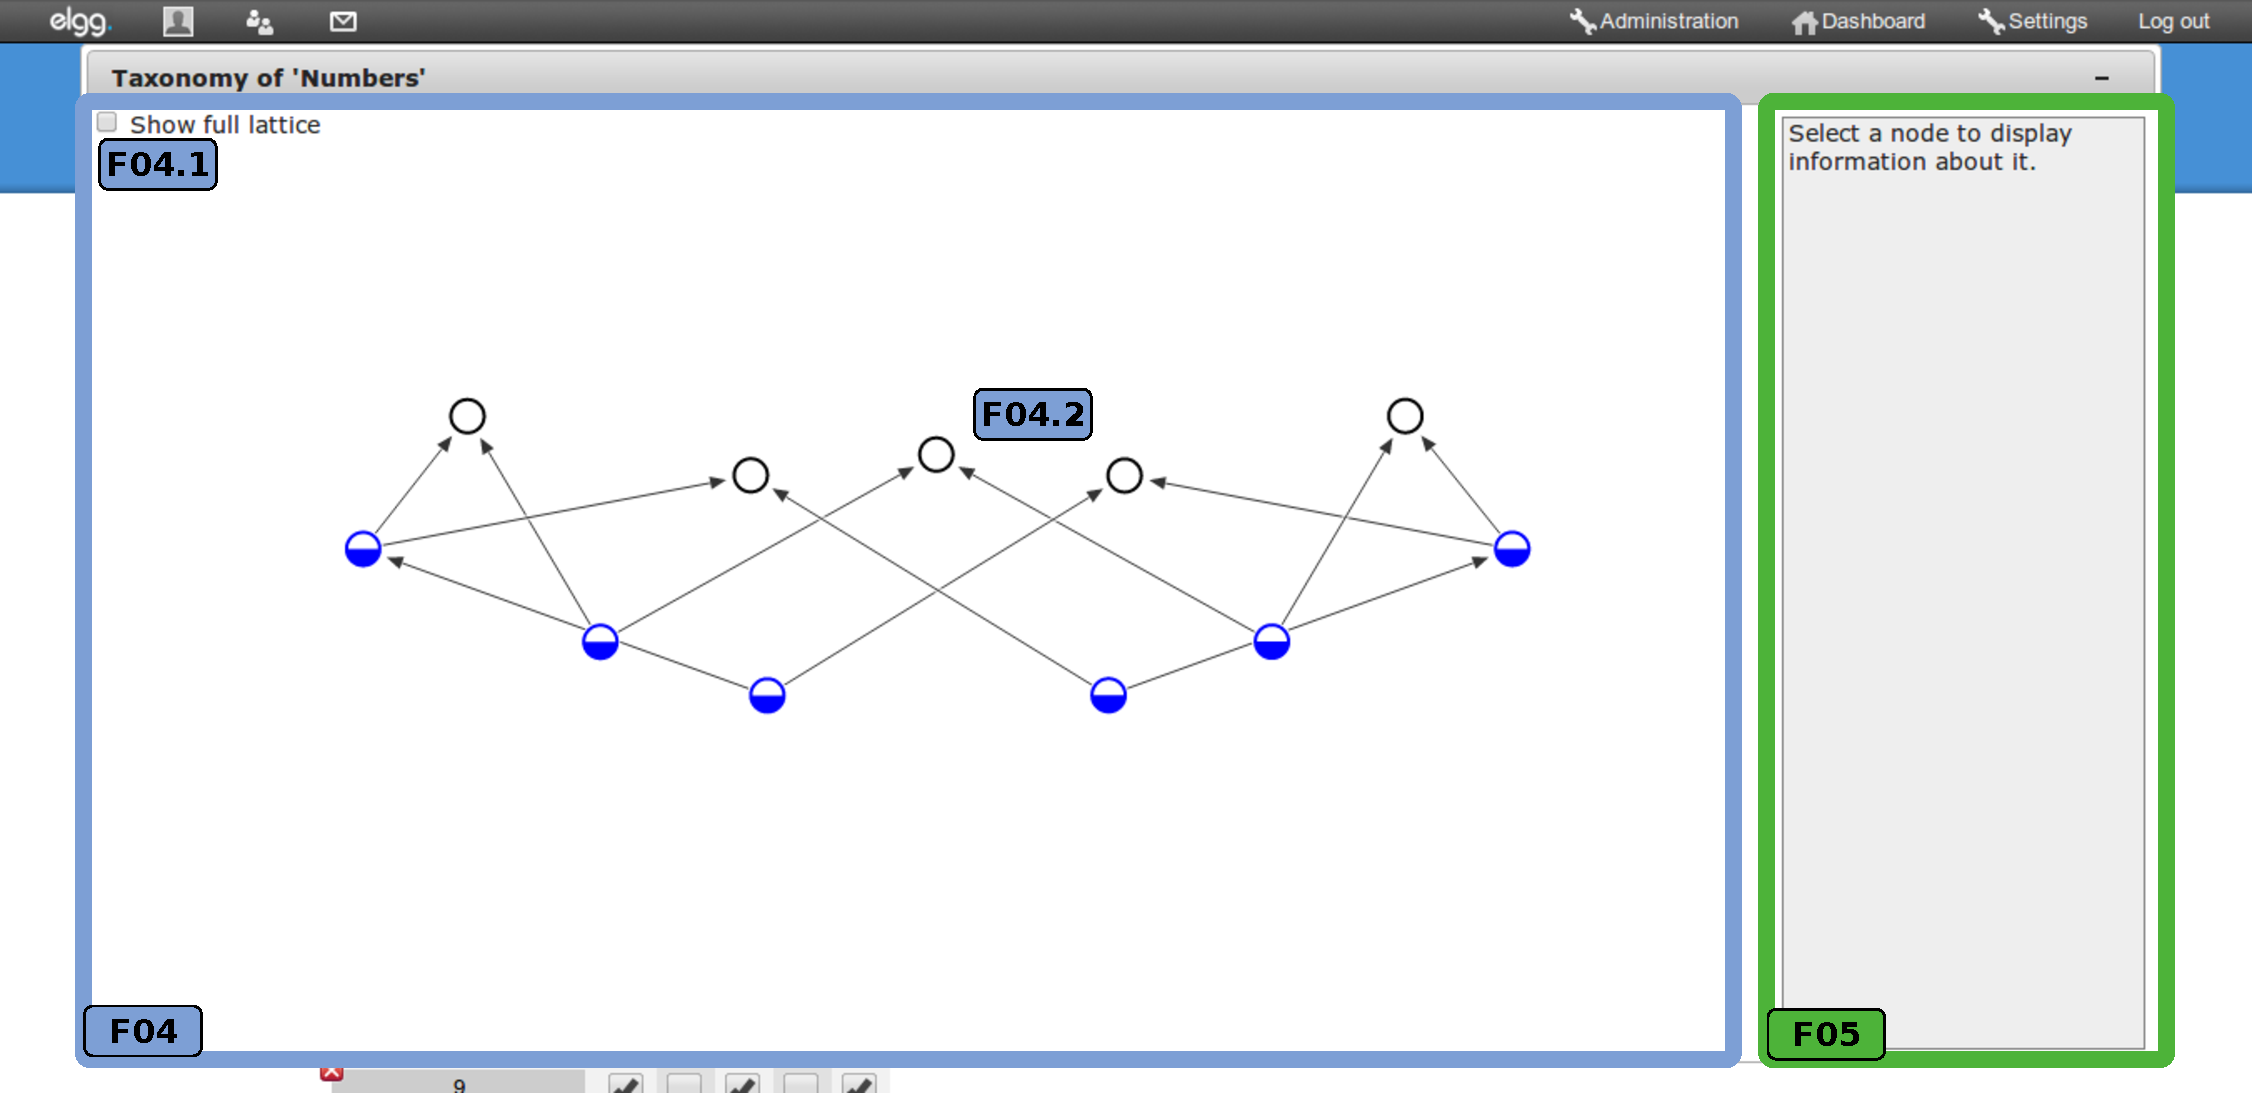
\includegraphics[width=\textwidth]{figures/taxonomy_show}
    \caption{Taxonomy}
    \label{fig:fca-lattice-view}
    \end{center}
  \end{subfigure}
  \begin{subfigure}{0.8 \textwidth}
    \begin{center}
    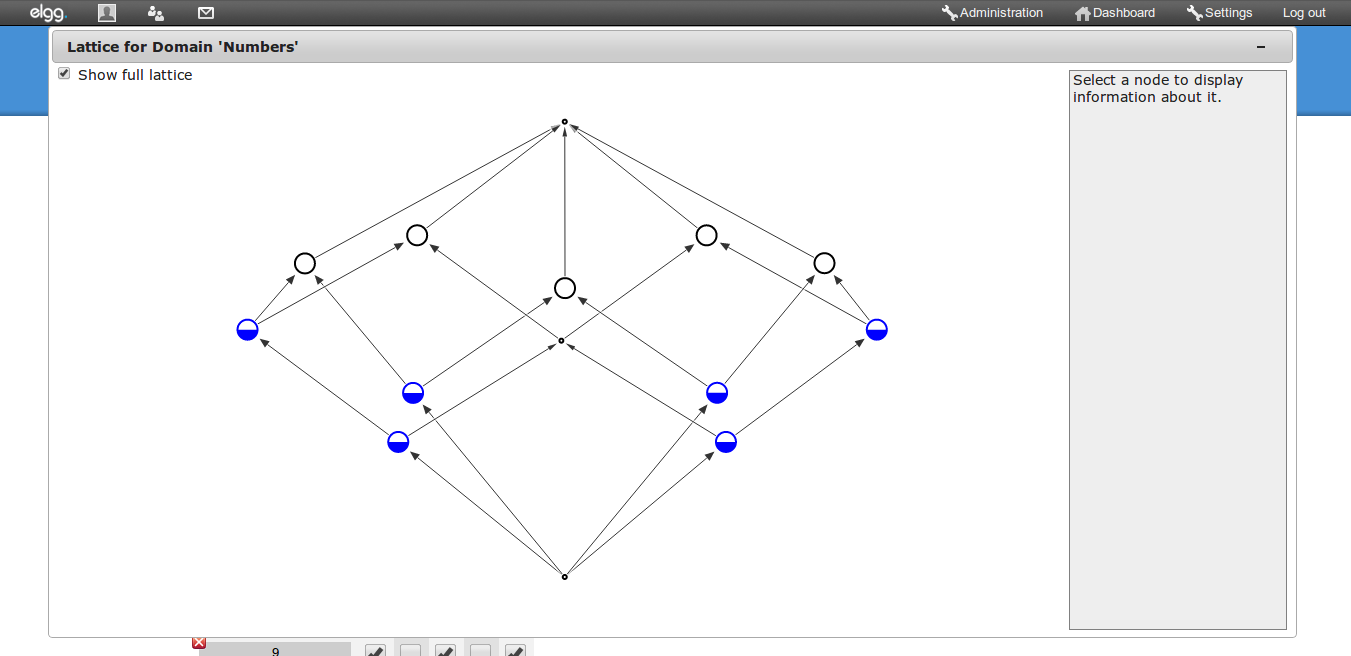
\includegraphics[width=\textwidth]{figures/lattice}
    \caption{Complete Formal Context}
    \label{fig:fca-lattice}
    \end{center}
  \end{subfigure}
\end{center}
\caption{Lattice View}
\end{figure}
\begin{figure}[h]
\begin{center}
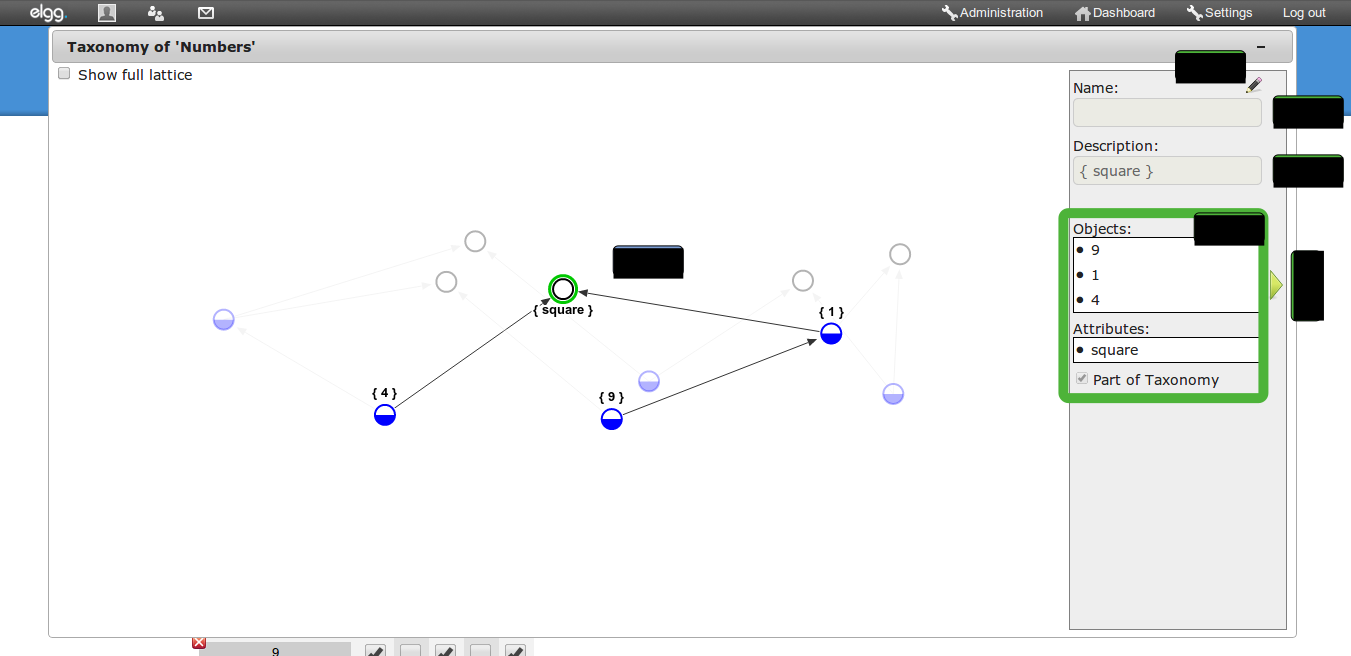
\includegraphics[width=0.8\textwidth]{figures/taxonomy_select}  
\end{center}
\caption{Selecting a Concept}
\label{fig:fca-taxonomy-sel}
\end{figure}

\begin{figure}[h]
\begin{center}
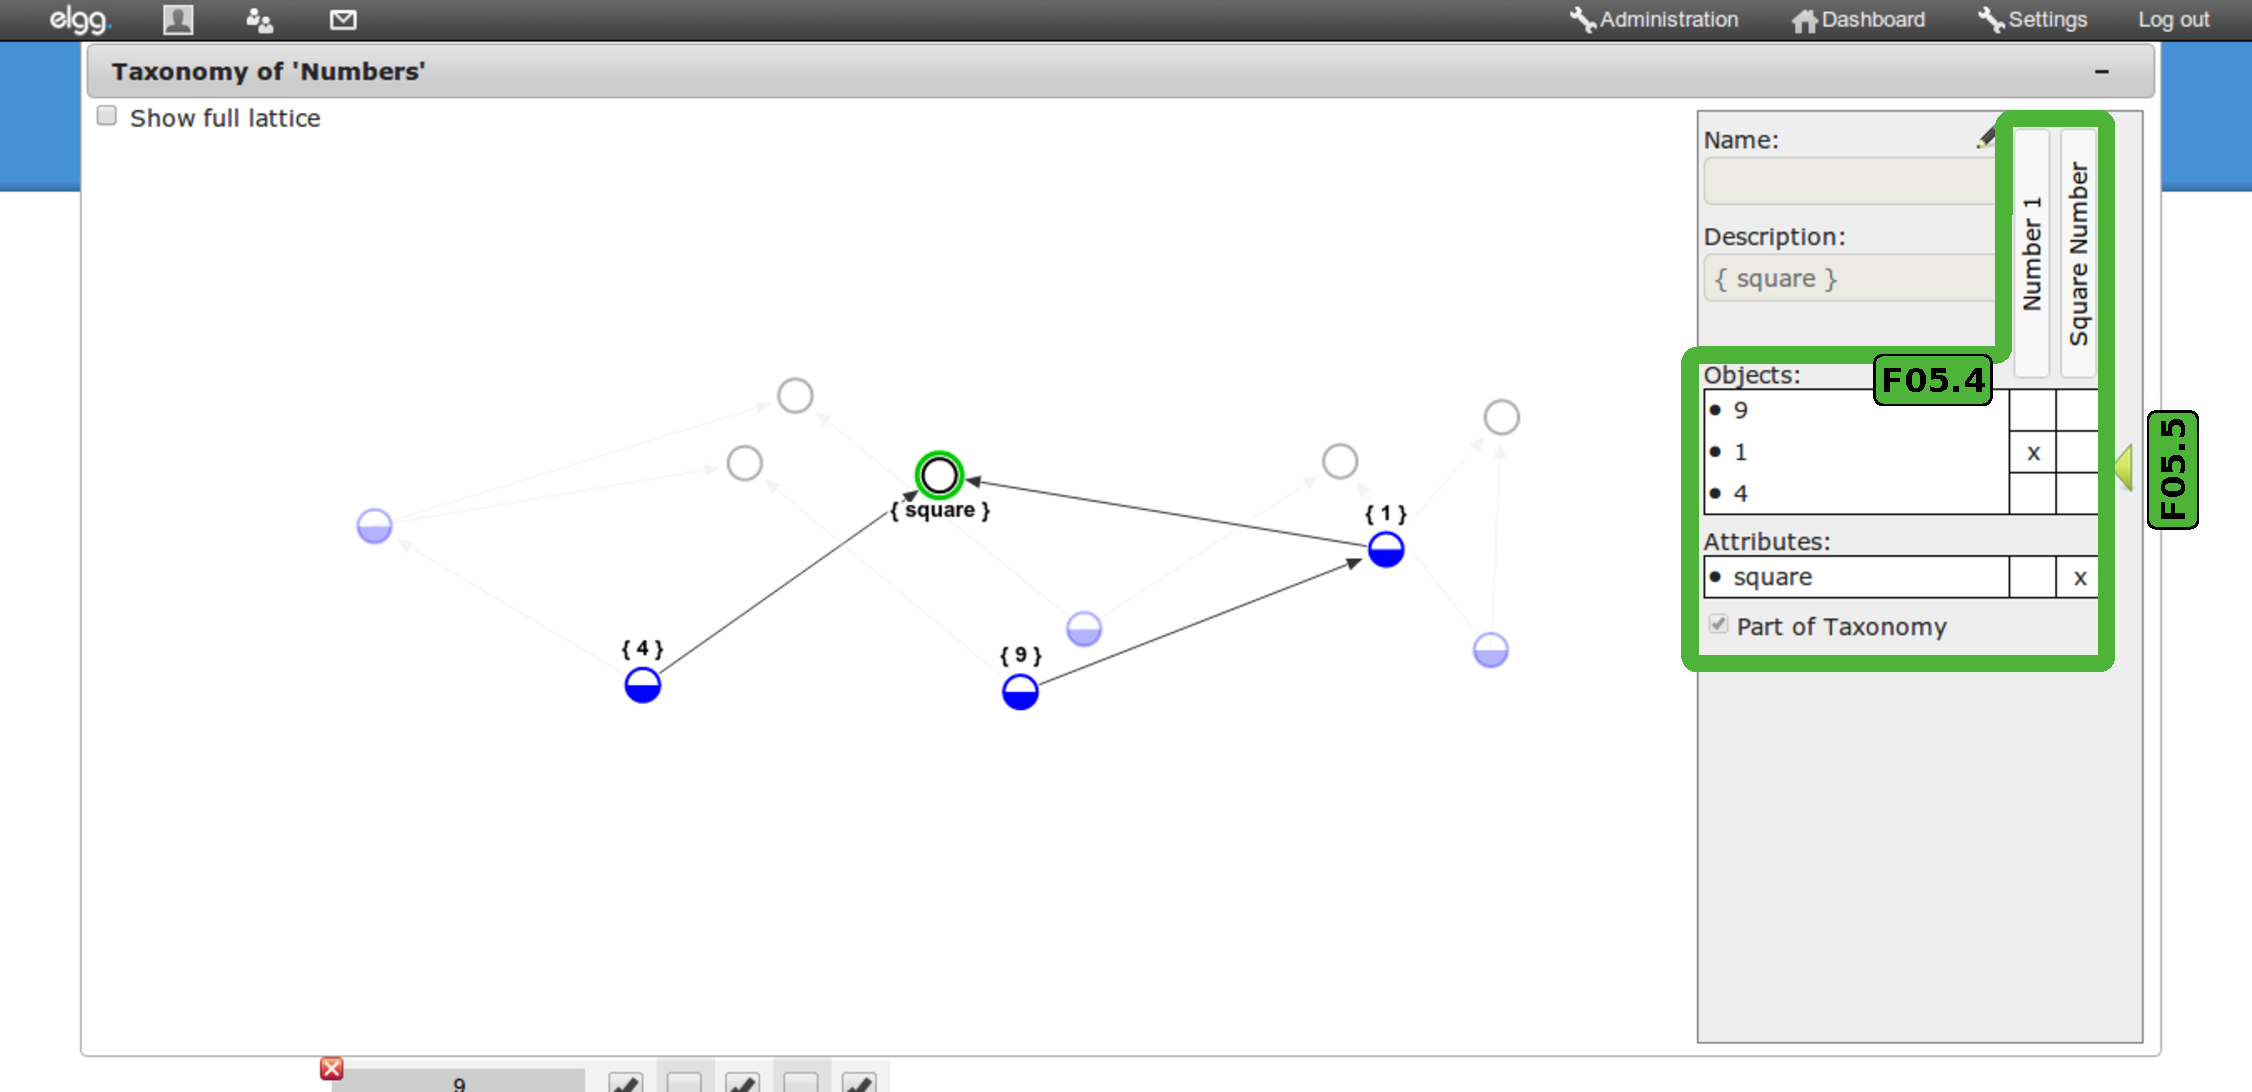
\includegraphics[width=0.8\textwidth]{figures/taxonomy_lo}  
\end{center}
\caption{Concept Learning Objects}
\label{fig:fca-taxonomy-lo}
\end{figure}
The individual concepts of the lattice can be dragged and clicked displaying labels and populating the side pane with the data of this concept (see Figure \ref{fig:fca-taxonomy-sel}). The side pane then features text fields containing the name \textbf{[F05.2]} and description \textbf{[F05.3]} of the selected concept and a section containing a list of objects and attributes the concept consists of  as well as an indicator if the concept is part of the taxonomy \textbf{[F05.4]}. Furthermore buttons to edit the concept \textbf{[F05.1]} and display the concept's learning objects \textbf{[F05.5]} are present.
Upon clicking the button \textbf{[F05.5]} the list of objects and attributes is extended into a matrix \textbf{[F05.4]} showing which learning objects are associated to which objects and attributes (see Figure \ref{fig:fca-taxonomy-lo}). The learning objects are again clickable opening a new tab containing the resource a learning object points to. Clicking teh button \textbf{[F05.5]} a second time hides the learning object matrix.
\paragraph*{Editing Concepts\\}
When clicking button \textbf{[F05.1]} the text fields containing name \textbf{[F05.2]} and description \textbf{[F05.3]} become editable, the check box of the indicator of section \textbf{[F05.4]} becomes clickable and a button \textbf{[F05.6]}  to save any changes made becomes visible (see Figure \ref{fig:fca-taxonomy-edit}).\\
The concept's objects, attributes as well as their learning objects cannot be modified.
\begin{figure}[h]
\begin{center}
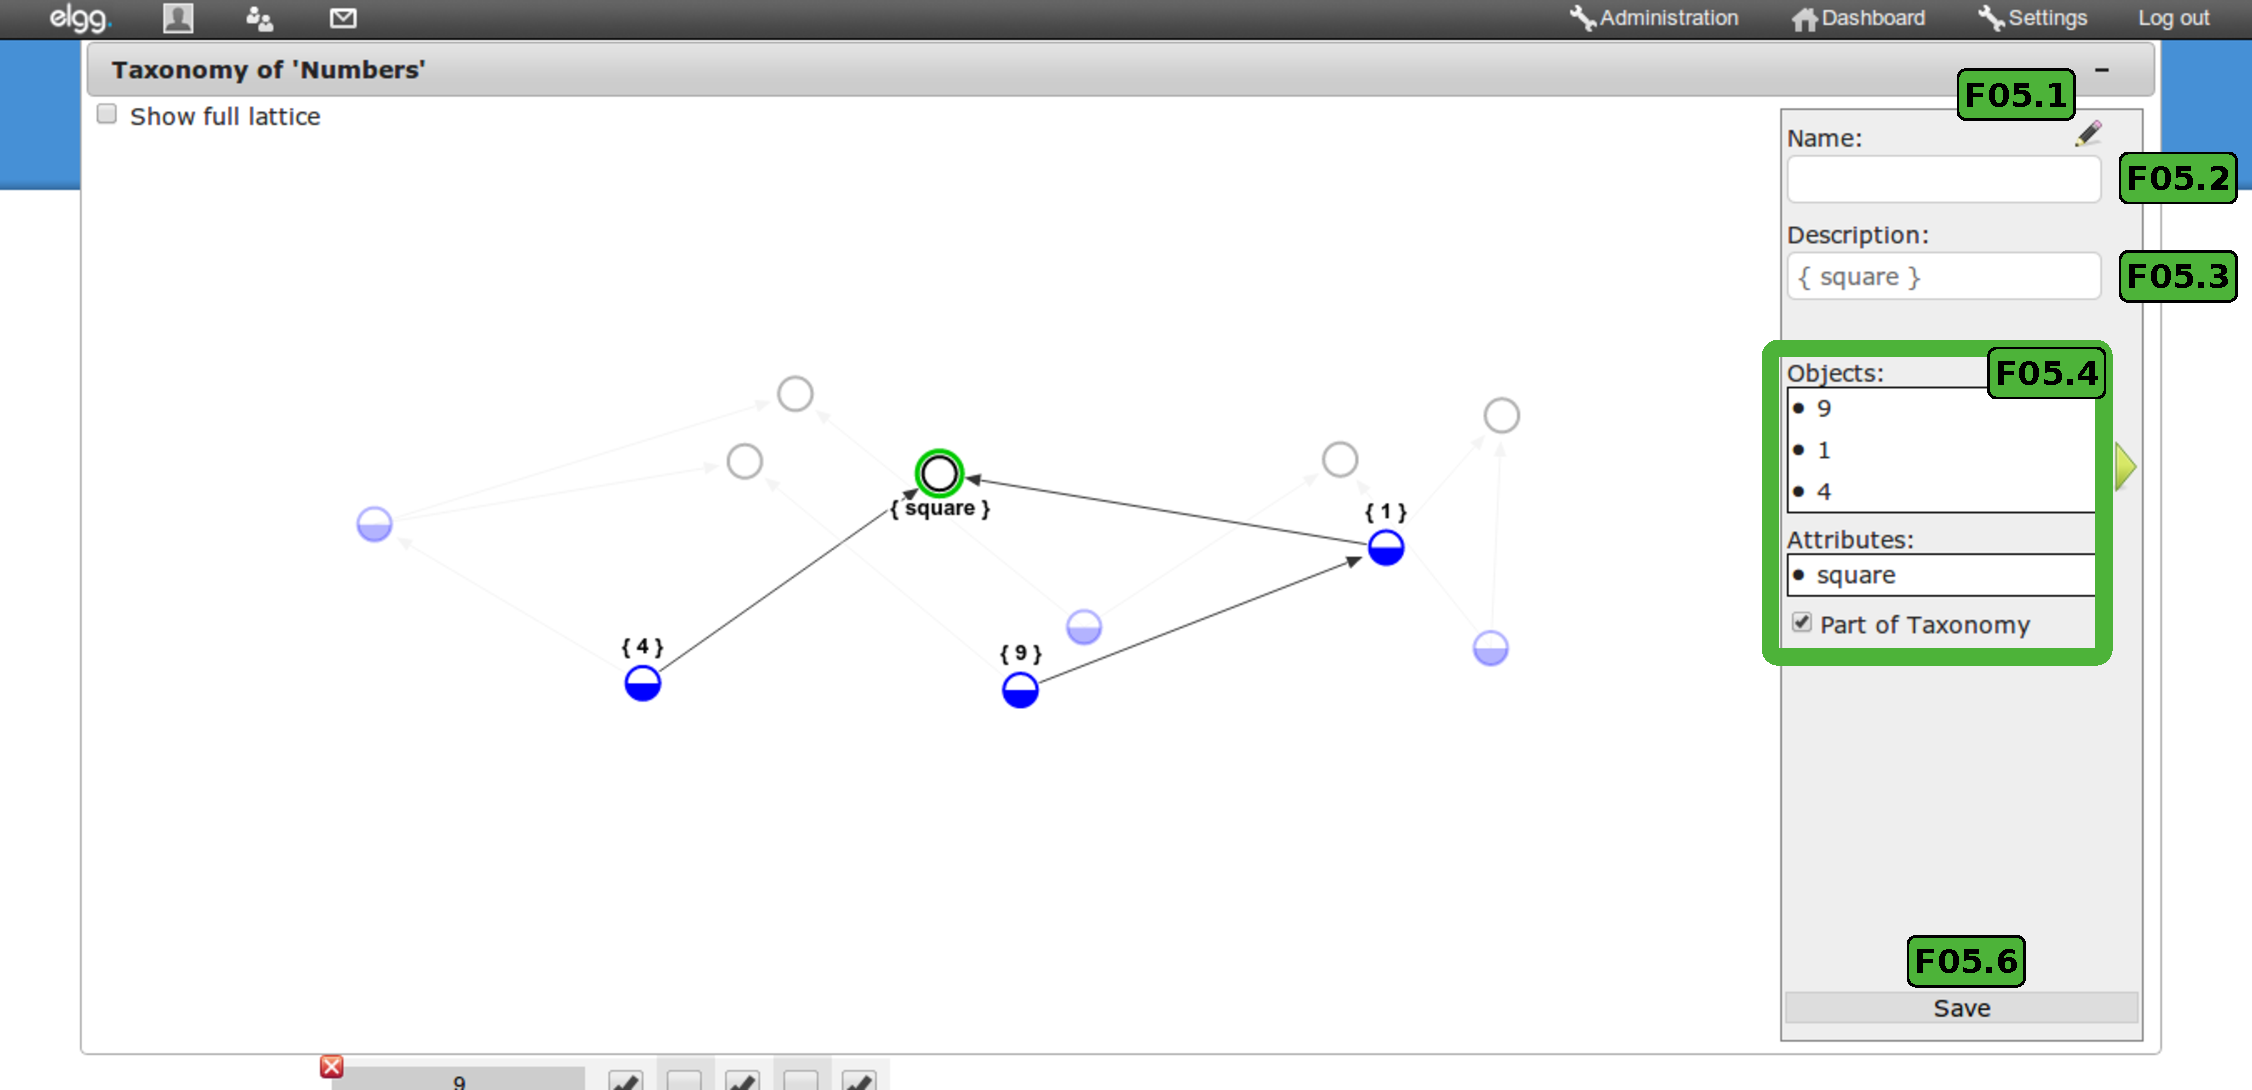
\includegraphics[width=0.8\textwidth]{figures/taxonomy_edit}  
\end{center}
\caption{Editing A Concept}
\label{fig:fca-taxonomy-edit}
\end{figure}
\end{document}
